\section{Methods and Materials}
% Here you should describe the design of your solution, your
% technical decisions, and why you believe your solution is appropriate. Some general
% images are recommended to enhance your explanation, and this section is expected
% to be 1 to 2 pages long. It is not recommended to include code here, but if you are
% presenting a complex algorithm, you may add it. Remember to write full paragraphs,
% with one idea per paragraph, and avoid using itemized lists. Aim for clarity and
% readability.

\subsection{System Architecture and Design}

Our approach to autonomous racing centers on a systems engineering methodology that integrates perception, decision-making, and control through a unified machine learning framework. We began by drawing a component diagram to show how each part of our system fits together (see Fig. \ref{fig:component_diagram}). This diagram clarifies the relationships between our sensor inputs, the learning agent, and the robot's control outputs before describing the technical details.


We began by drawing a component diagram to show how each part of our system fits together (see Fig. \ref{fig:component_diagram}). This diagram clarifies the relationships between our sensor inputs, the learning agent, and the robot’s control outputs before describing the technical details.

\begin{figure}[h]
    \centering
    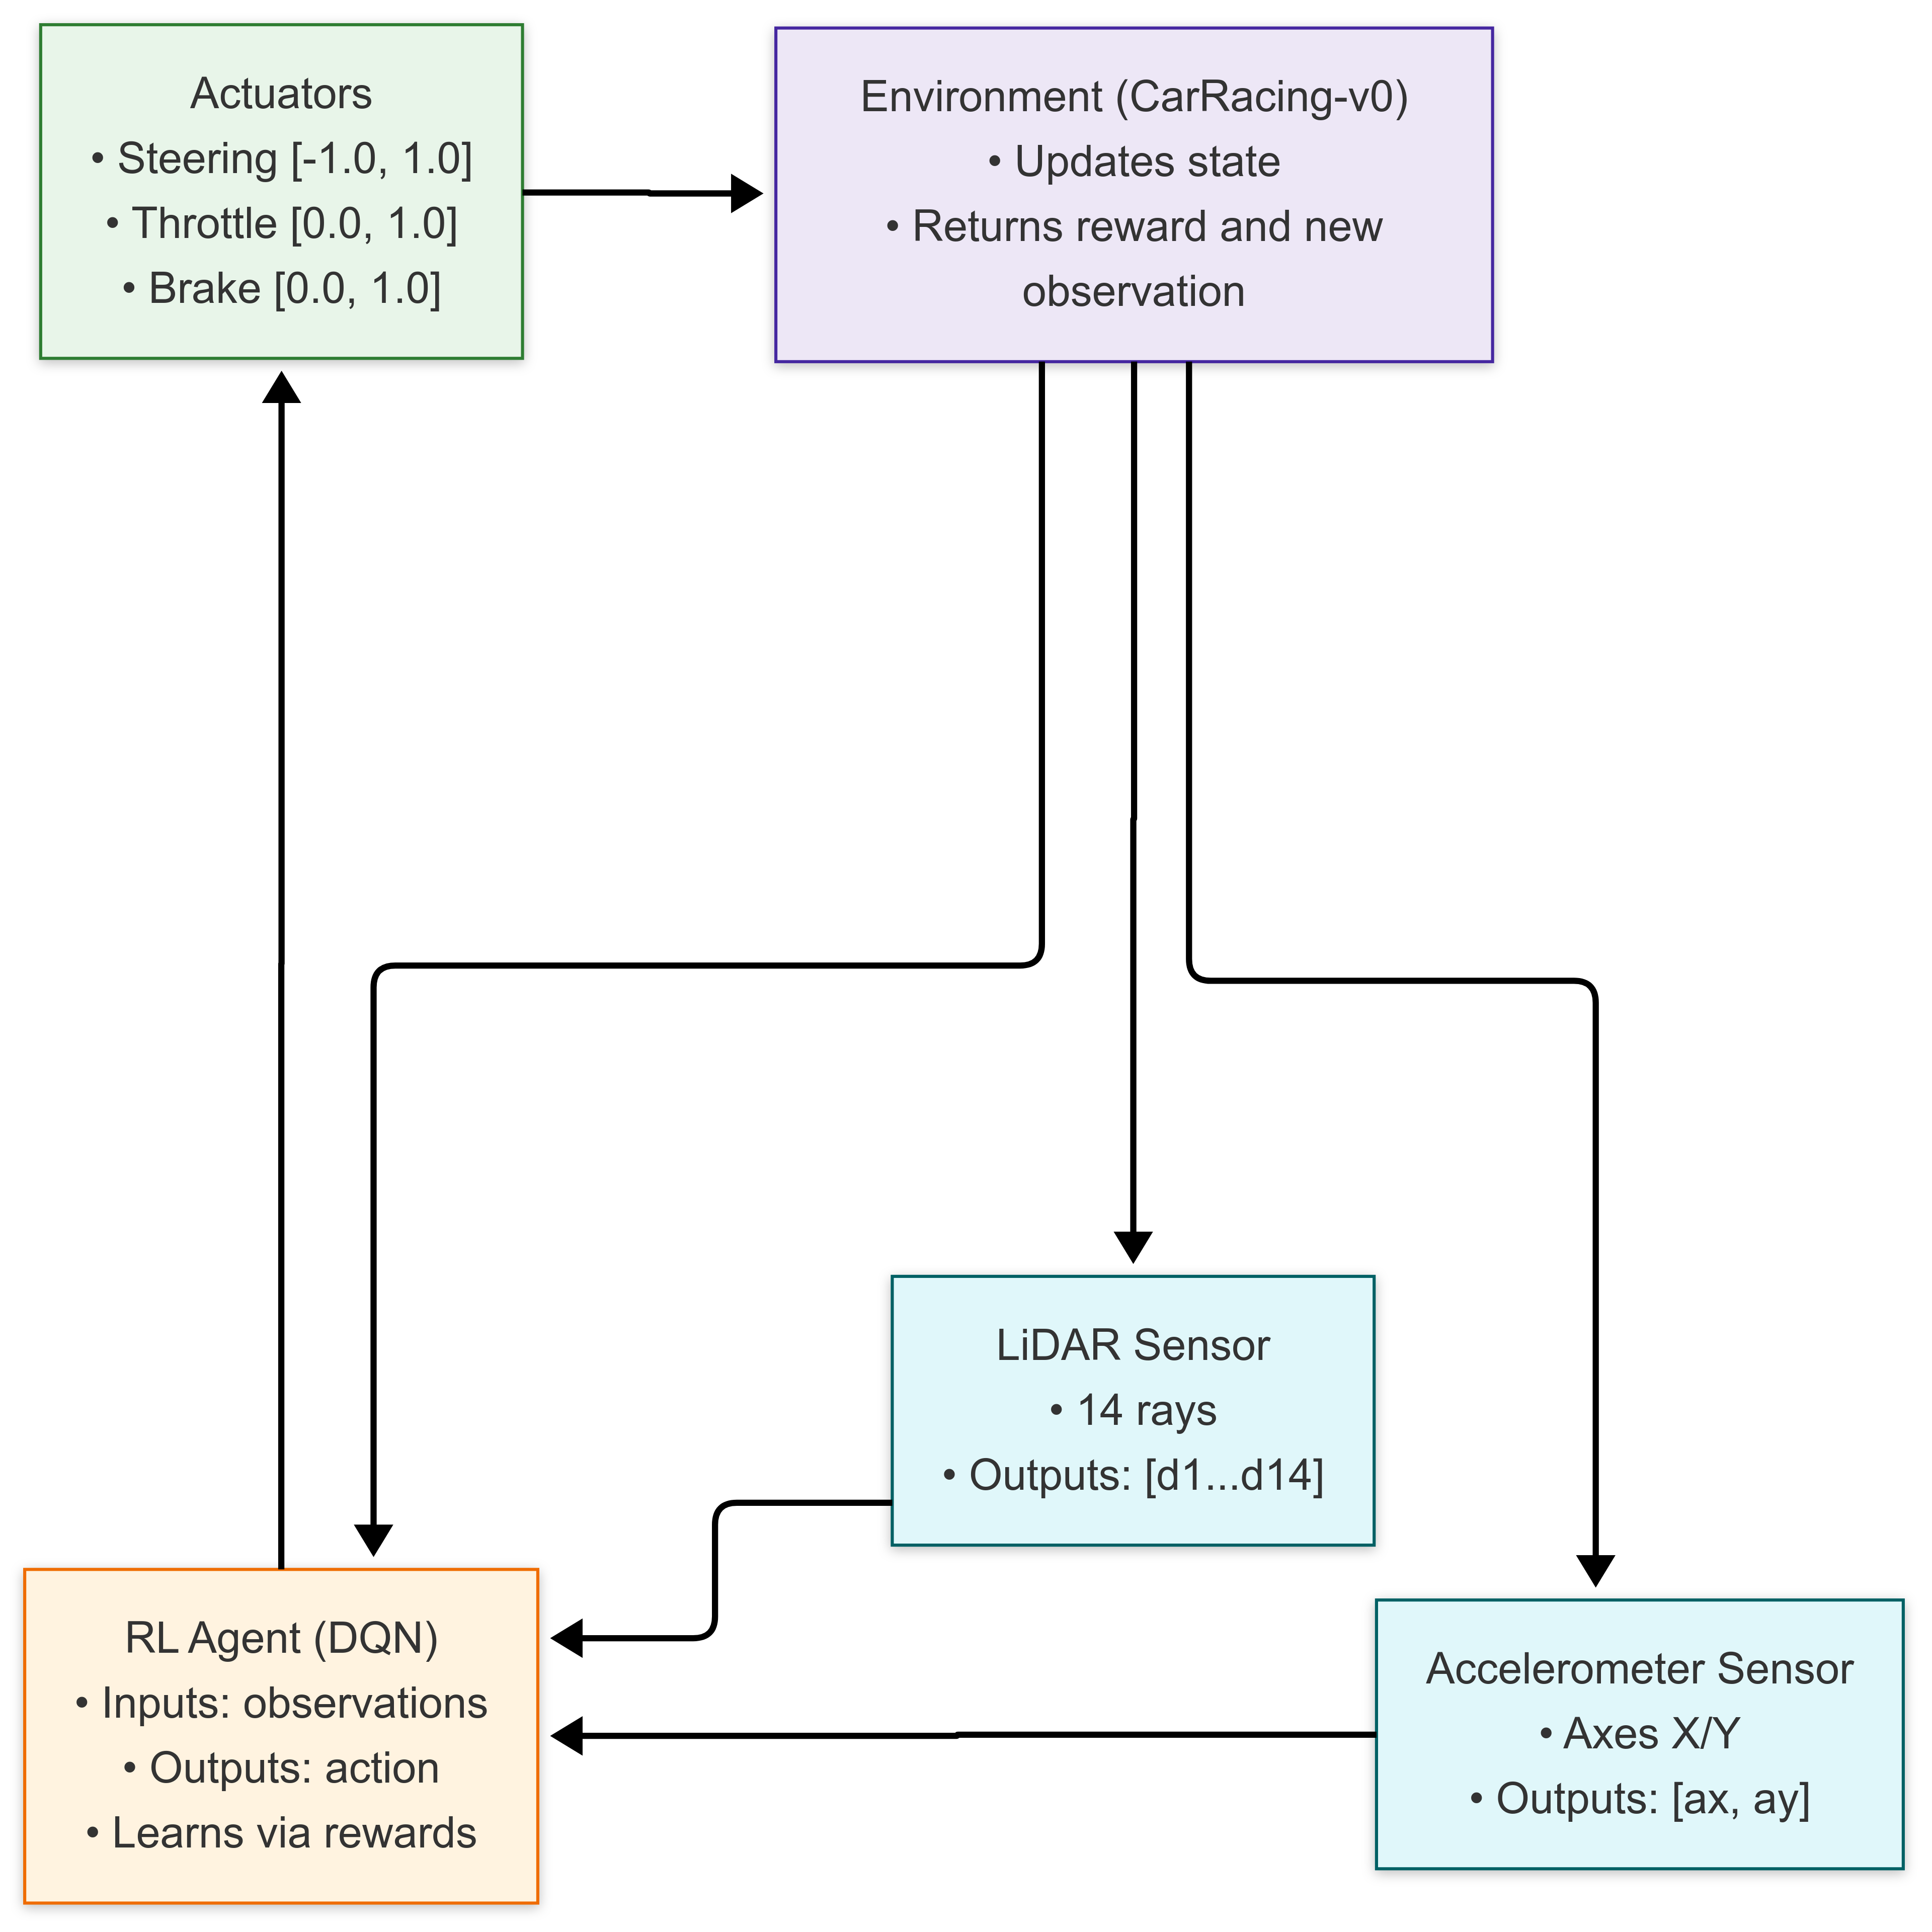
\includegraphics[width=0.8\linewidth]{images/ComponentDiagram.png}
    \caption{Component diagram of the system.}
    \label{fig:component_diagram}
\end{figure}

Our system design leverages the CarRacing-v3 environment from Gymnasium, which provides a two-dimensional, top-down view of a procedurally generated racetrack. At each time step, the agent receives a single 96×96 RGB image showing the car at the center of the track. In addition to this visual input, Gymnasium exposes four ABS sensor readings (one for each wheel), true speed, steering position, and gyroscope measurements. We combine these data into a single state representation that the agent observes.


\subsection{Deep Q-Network Implementation and Technical Framework}

To navigate and avoid obstacles, we implemented a Deep Q-Network (DQN) agent following a systematic approach to algorithm selection and implementation. Our technical framework prioritizes reproducibility and compatibility through careful version control and dependency management.

We employ Python 3.10 with the miniconda distribution of Anaconda for simplified dependency management. Rather than developing a custom environment from scratch, we leverage the prebuilt CarRacing-v3 environment from the gymnasium library. For the DQN implementation, we utilize StableBaselines3, which provides a robust and well-tested implementation of the algorithm. The following table presents the specific versions used to ensure compatibility and reproducibility:

\begin{center}
\begin{tabular}{ll}
  \textbf{Python Version:} & 3.10.16 \\
  \textbf{Torch Version:} & 2.7.0 \\
  \textbf{Gymnasium Version:} & 1.1.1 \\
  \textbf{Numpy Version:} & 2.0.1 \\
  \textbf{Scipy Version:} & 1.15.3 \\
  \textbf{Swig Version:} & 4.3.1 \\
  \textbf{Stable Baselines3 Version:} & 2.6.0 \\
  \textbf{IPython Version:} & 8.30.0 \\
\end{tabular}
\end{center}

The DQN uses a convolutional neural network to approximate the action-value function over continuous control actions—steering, gas, and brake. During training, the agent’s experiences (state, action, reward, next state) are stored in a replay buffer. We periodically sample mini-batches from this buffer to update the main network, while a separate target network—updated every few episodes—helps stabilize learning.

The reward function, provided by the Gymnasium CarRacing-v3 environment \cite{gymnasium2023}, is designed to encourage both speed and track coverage. At each frame, the agent receives a \(-0.1\) penalty, which pushes it to finish the track quickly. Each newly visited track tile yields a bonus of \(1000/N\) points, where \(N\) is the total number of tiles. For example, covering all tiles in 732 frames yields:
\[
    1000 - 0.1 \times 732 \approx 926.8 \text{ points}.
\]
Crashing off-track for too long or failing to visit new tiles ends the episode.

\begin{figure}[h]
    \centering
    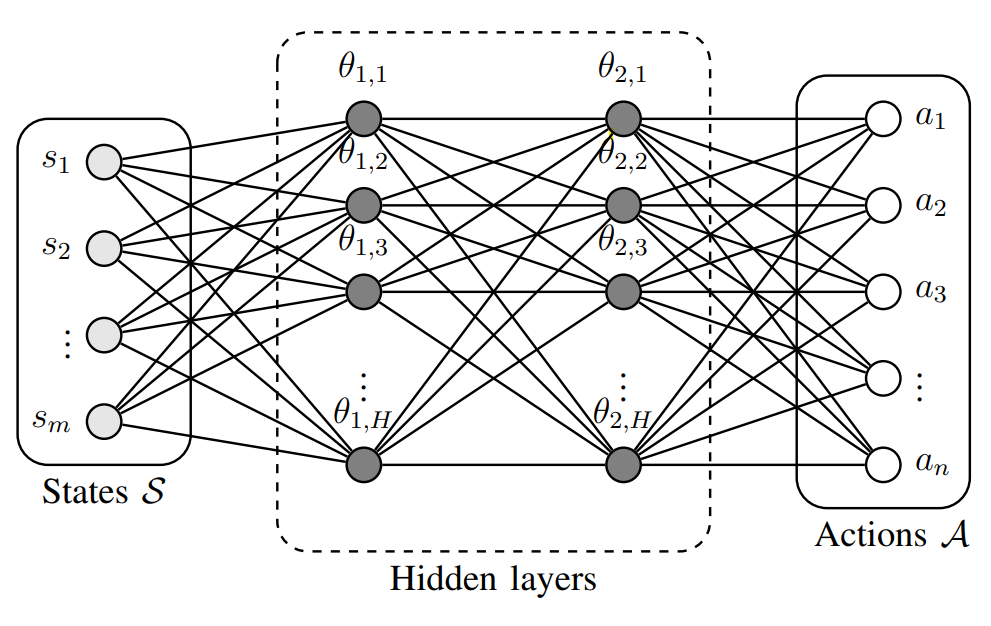
\includegraphics[width=0.8\linewidth]{images/DQNmodel.png}
    \caption{DQN algorithm diagram \cite{DQNimage}.}
    \label{fig:dqn_diagram}
\end{figure}

Figure \ref{fig:dqn_diagram} illustrates the overall DQN workflow. In our implementation, the input image and sensor readings pass through convolutional and fully connected layers to produce Q-values for each action. The action with the highest Q-value is selected at each step. Over thousands of episodes, the agent learns to balance acceleration, braking, and steering to maximize cumulative reward while avoiding track boundaries.

\subsection{Cybernetic Feedback Integration and Sensor Processing}

The integration of cybernetic feedback in our DQN agent represents a critical aspect of the system design. Rather than explicit programming of sensor-to-reward mappings, our approach achieves this integration through structured learning processes that map environmental perception to decision-making.

The agent's primary sensory input consists of raw RGB images (96×96 pixels) from the racing environment. To optimize training efficiency and reduce computational overhead, we implement a sophisticated preprocessing pipeline. The input images are converted to grayscale and resized to 84×84 pixels using the WarpFrame wrapper. To capture temporal dynamics such as speed, orientation, and trajectory, four consecutive frames are stacked using VecFrameStack, providing the agent with short-term visual memory essential for motion-aware decision making.

The reward structure in CarRacing-v3 is predefined by the environment, eliminating manual engineering bias. The agent learns to associate patterns in processed observations with delayed environmental feedback, enabling the development of strategies that maximize cumulative reward over time. The following tables illustrate the conceptual framework of environmental data interpretation and action-feedback integration within our system.

\begin{table}[h!]
\caption{Environmental Data and Agent Perception}
\label{tab:env_perception_en}
\centering
\footnotesize
\begin{tabular}{|p{2.8cm}|p{4.5cm}|}
\hline
\textbf{Environmental Aspect} & \textbf{Agent's Perceptual Basis} \\
\hline
Car position/orientation & Visual patterns, lane markings, track edges from stacked grayscale frames \\
\hline
Speed and momentum & Frame-to-frame changes and visual speedometer cues \\
\hline
Track layout & CnnPolicy feature extraction for geometry anticipation \\
\hline
Track boundaries & Visual distinction between track surface and off-track areas \\
\hline
Dashboard indicators & Visual features for car's internal state information \\
\hline
\end{tabular}
\end{table}

\begin{table}[h!]
\caption{Action-Feedback Integration}
\label{tab:reward_integration_en}
\centering
\footnotesize
\begin{tabular}{|p{2.2cm}|p{2.3cm}|p{2.8cm}|}
\hline
\textbf{Agent Action} & \textbf{Reward Signal} & \textbf{Learning Impact} \\
\hline
Appropriate steering/acceleration & +1000/N per tile visited & Reinforces successful progression \\
\hline
Incorrect steering, excessive speed & -100 penalty & Discourages undesirable outcomes \\
\hline
Any action per timestep & -0.1 per step & Encourages efficiency \\
\hline
Effective control use & Higher cumulative rewards & Learns optimal strategies \\
\hline
\end{tabular}
\end{table}

This systematic approach to cybernetic feedback demonstrates the information flow from raw sensory data, through processing stages, to decision-making, with environmental feedback closing the loop to enable adaptive behavior based on the objectives defined within the CarRacing-v3 environment.

By combining visual information with sensor data and training with the DQN algorithm in the CarRacing-v3 environment, our system learns to navigate complex tracks efficiently and safely. This modular design approach provides a foundation for future extensions, including integration of additional perception modules or deployment on physical robotic platforms.

\subsection{System Behavior Analysis and Perturbation Response}

To evaluate the robustness and adaptability of our DQN agent, we conduct systematic analysis of system behavior under various perturbations and environmental conditions. This analysis framework examines how the agent responds to dynamic changes in the racing environment and identifies the stability boundaries of the learned control policies.

Our perturbation analysis considers three primary categories of disturbances: environmental perturbations (track surface conditions, lighting variations), dynamic perturbations (sudden velocity changes, steering noise), and sensor perturbations (temporary vision occlusion, sensor drift). Each perturbation type is systematically introduced during testing phases to assess the agent's resilience and recovery capabilities.

The behavioral analysis employs phase space reconstruction techniques to visualize the agent's decision-making patterns. By plotting the agent's actions against environmental states over time, we can identify stable behavioral attractors, transition dynamics, and potential instability regions. This approach provides insights into the emergent control strategies developed by the DQN algorithm and helps validate the system's performance boundaries.

We implement a real-time monitoring system that tracks key performance indicators including steering smoothness, velocity consistency, track adherence, and recovery time from off-track incidents. These metrics provide quantitative measures of system stability and enable comparison between different training configurations and environmental conditions.

\begin{table}[h!]
\caption{Perturbation Categories and System Response Metrics}
\label{tab:perturbation_analysis}
\centering
\footnotesize
\begin{tabular}{|p{2.5cm}|p{2.0cm}|p{2.8cm}|}
\hline
\textbf{Perturbation Type} & \textbf{Test Conditions} & \textbf{Response Metrics} \\
\hline
Environmental & Track surface changes, lighting variations & Track adherence, lap completion rate \\
\hline
Dynamic & Velocity changes, steering noise & Stability index, recovery time \\
\hline
Sensor & Vision occlusion, sensor drift & Adaptation rate, performance degradation \\
\hline
System & Network updates, policy changes & Convergence stability, learning efficiency \\
\hline
\end{tabular}
\end{table}

This table categorizes the perturbations introduced during the analysis and the corresponding metrics used to evaluate the system's response. By systematically testing and analyzing these perturbations, we gain insights into the strengths and limitations of the learned DQN policies and identify opportunities for further improvement and optimization.

